\chapter{Realization}

\section{Planning}
The first phase of the project was the planning phase. In this phase I researched existing solutions and defined the requirements for the project. I also planned the hardware and software setup for my project. This included defining the components, the software stack and the data flow.

\subsection{Requirements}
To start of this project I had to define a set of requirements that the solution should fulfill. These requirements were then used to guide the design of the solution. I sat down with my family member and discussed the functional and non-functional requirements. The functional requirements were the features that the solution should have. The non-functional requirements were the requirements that were not directly related to the functionality of the solution.

\newpage
\subsection{Functional Requirements}
\begin{itemize}
    \item The solution should be able to be deployed in any location.
    \item The solution should include its own power supply.
    \item The solution should be able to connect to the internet in a location independent manner.
    \item The solution should be able to measure the weight of the beehive.
    \item The solution should be able to measure the temperature of the beehive.
    \item The solution should publish the data it collects to the internet.
    \item The solution should save the data it collects in a persistent manner.
    \item The solution should not require any special equipment to be installed.
    \item The solution should be able to be installed in a standard beehive.
    \item The solution should be implementation independent. Meaning that the individual components can be replaced with other components that fulfill the same function.
\end{itemize}
\subsection{Non-Functional Requirements}
\begin{itemize}
    \item The solution should be as energy efficient as possible.
    \item The solution should be able to generate its own power.
    \item The solution should be resistant to the elements.
    \item The solution should be as cost-effective as possible.
    \item The solution should be simple to build.
    \item The solution should be easy to maintain.
    \item The solution should be easy to extend.
\end{itemize}

\newpage
\subsection{Current Solutions}
It was important for me that I did not reinvent the wheel and add something to the existing solutions. I therefore researched existing solutions and compared them to my requirements. I found that there are a lot of solutions for beekeepers. Most of them are either very expensive or very complex. I also found that most of the solutions are not open source. This means that the data is not accessible to the beekeeper. This is a problem because the beekeeper should be able to access the data and analyze it in the way they want to and not rely on any proprietary solutions that might not provide them with the information they need. Furthermore, most of the solutions are not modular. This means that the beekeeper is not able to add new sensors or actuators to the system. This is a problem because the beekeeper should be able to add new sensors and actuators to the system. Most of the solutions are also unreasonably expensive and bind the user to a subscription. This means that the beekeeper has to invest a lot of money into the system that doesn't have an obvious return of investment.

\newpage
\subsubsection{HiveWatch}

\begin{figure}
    \centering
    
\includegraphics[width=0.75\textwidth]{figures/hivewatch_logo.png}
    \caption{HiveWatch}
    \label{fig:hivewatch}
\end{figure}
HiveWatch is a swiss-made, all in one solution to measure the weight of a beehive. It consists of a "transmitter" that can connect up to 8 scales that are also sold by the company. This seems to be done with a proprietary connector that isn't documented very well. It uses a 4G/LTE-M connection to connect to the internet.

\begin{figure}
    \centering
    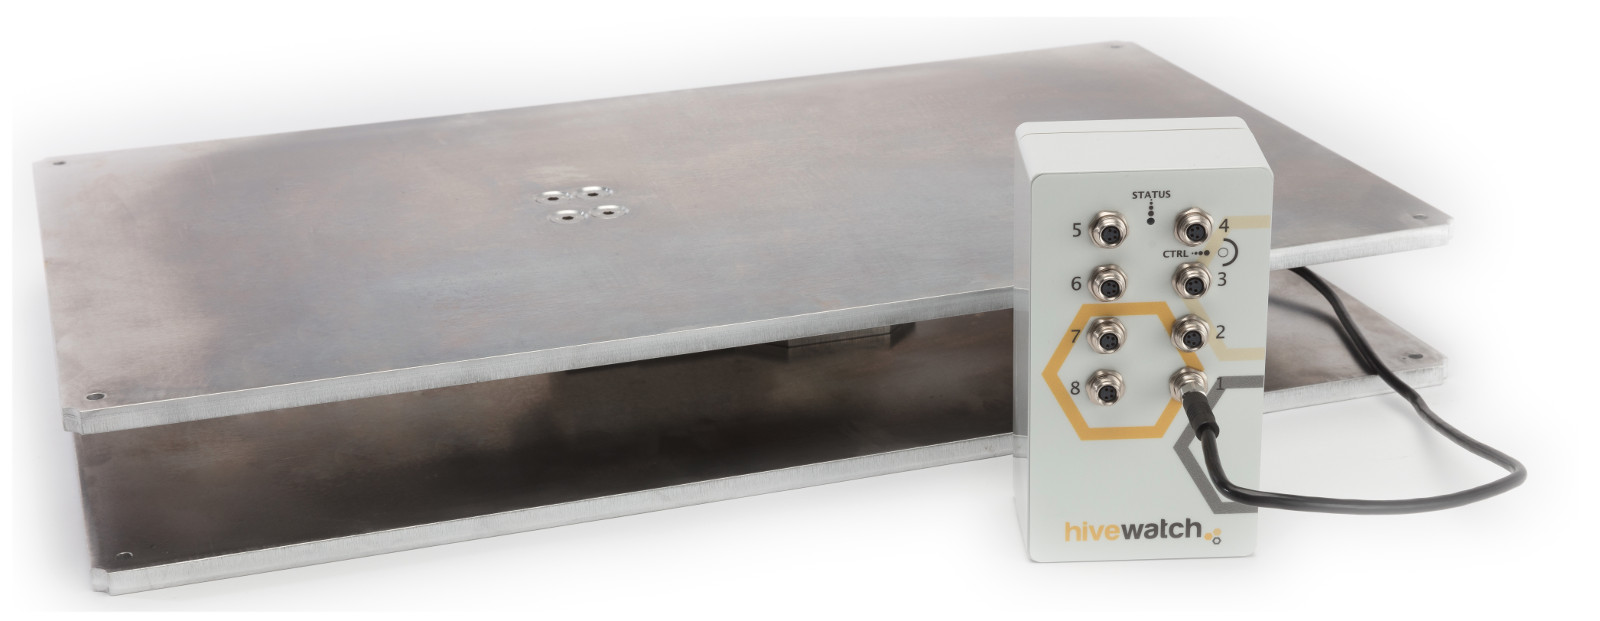
\includegraphics[width=0.75\textwidth]{figures/hivewatch_scale.jpg}
    \caption{HiveWatch System}
    \label{fig:hivewatch_scale}
\end{figure}

\textbf{Price:}
\begin{table}[ht]
    \centering
    \begin{bfhTabular}{lll}
       Expense & Price
       \\\hline
       Transmitter & CHF \num{385.00}\\\hline
       Scale & CHF \num{204.00} & \\\hline
       Brood Humidity Sensor & CHF \num{65.00}\\\hline
       Extension Cable & CHF \num{19.00} & \\\hline
       Subscription for 1 year & CHF \num{89.00}\\\hline
       \textbf{Total} &  \textbf{CHF 862.00}
    \end{bfhTabular}
    \caption{Price HiveWatch system}
    \label{tab:hivewatch_price}
 \end{table}

\newpage
\textbf{Interesting Features:}
\begin{itemize}
    \item HiveWatch is a modular system withing its own ecosystem. New scales can be added to the system with a proprietary connector. It seems like extending this system is plug-and-play.
    \item HiveWatch provides an app that can be used to monitor the weight of the beehive. The app also provides a history of the measured data.
    \item The beekeeper can set up alerts that will notify them if certain events occur. This includes, for example, if the scale thinks it detects a bee swarm.
\end{itemize}
\textbf{Problems:}
\begin{itemize}
    \item HiveWatch is a closed system. Interfaces are not documented, and the data is not accessible to the beekeeper by default. There is a forum where you can ask questions about the system. The developer seems to be reasonably active and provides information about the system, but this is not a good solution.
    \item It seems that the data is only accessible through the app. This makes it hard to analyze the data in a way that isn't intended by the developer.
    \item The solution is very expensive. The system also only seems to work if you have a subscription which is also very expensive.
\end{itemize}
\newpage

\subsubsection{Wolf-Waagen}

\begin{figure}
    \centering
    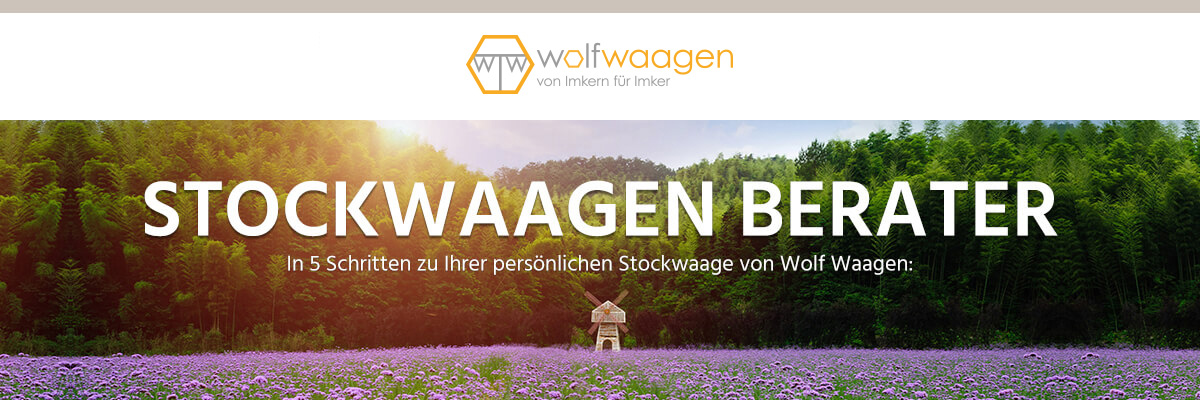
\includegraphics[width=1\textwidth]{figures/wolf_waagen_logo.jpg}
    \caption{Wolf-Waagen}
    \label{fig:wolf_waagen}
\end{figure}
Wolf-Waagen (Wolf-Scales) is a German business that specializes in bee scales. They sell a variety of scales that can be used to measure the weight of a beehive. They also have a diverse variety of sensors that can be used to collect additional data points like rainfall or wind. Furthermore, they provide a web interface that can be used to monitor the scales and provide an SMS altering service.

\begin{figure}
    \centering
    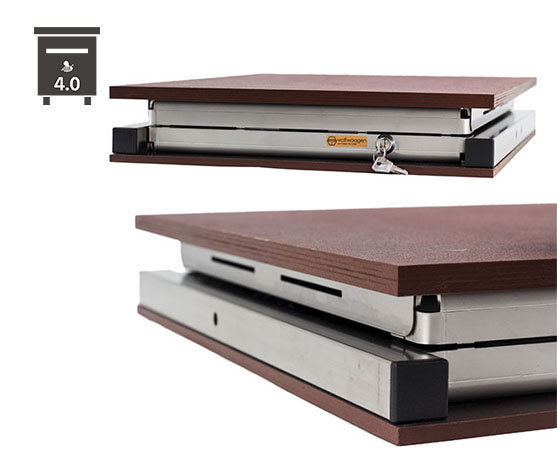
\includegraphics[width=0.75\textwidth]{figures/wolf_waagen_4.0.jpg}
    \caption{Wolf-Waagen System}
    \label{fig:wolf_waagen_4.0}
\end{figure}

\textbf{Price:}
Sadly, Wolf-Waagen doesn't give any exact information about pricing. They only specify the minimum price of the "ApiGraph4.0" scale, which is €\num{899.00}.
\begin{table}[ht]
    \centering
    \begin{bfhTabular}{lll}
       Expense & Price
       \\\hline
       ApiGraph4.0 & € \num{899.00}+\\\hline
       Software Service for 1 year & € \num{24.00} & \\\hline
       Data Plan for 1 year & € \num{15.00}\\\hline
       \textbf{Total} &  \textbf{CHF 938.00+}
    \end{bfhTabular}
    \caption{Price Wolf-Waagen system}
    \label{tab:tab1}
 \end{table}

\newpage
\textbf{Interesting Features:}
\begin{itemize}
    \item The scale appears to be really well-built. Most of the parts are made of metal and the scale looks really sturdy. Overall it seems like a good quality product. 
    \item Wolf-Waagen provides the option to connect additional sensors to the scale. It also seems like you can easily hook up additional scales to the system.
    \item They give you the option to have a diverse assortment of power sources. This includes solar panels, batteries, and a power adapter.
\end{itemize}
\textbf{Problems:}
\begin{itemize}
    \item Although the system seems to be really well-built, it is very expensive. The price of the scale is already very high, and the subscription and data plan are also very expensive.
    \item It looks like you have to completely rely on the Wolf-Waagen service. The data is not accessible to the beekeeper by default. The beekeeper can only access the data through the web interface. This makes it hard to analyze the data in a way that isn't intended by the developer.
\end{itemize}

\newpage

\subsection{Open Source Solutions}

There are a lot of open source projects that aim to solve the same problem. However, as with many open source projects, they are not very well documented and are not very easy to use. Also since they are often created by hobbyists, they are not general purpose solutions. They are often very specific to the needs of the creator. This makes it hard to use them in a real-world scenario.

Because of this, I decided to not use any of these solutions as is but to improve on existing concepts. I think that it is better to create my own solution easy to use and is suited to my needs.

\newpage

\subsection{Hardware Planning}
\subsubsection{Rough Setup}
In essence, the scale needs to provide a surface on which the beehive can be mounted and that measures the weight applied to it. This should be as low to profile as possible as not to interfere with any existing mounting equipment like standoffs or compartments in a bee house.

For this reason, I've decided to work with a simple, two plates approach. The first plate is the actual scale on which the beehive is mounted. The second plate is a baseplate to provide a stable foundation to the second plate. The load cells are mounted in between the two plates together with the load cell amplifier, so there is no need for any additional wiring and the scale can be connected to the microcontroller over a single cable.

The microcontroller is located in a separate housing, so it can be easily accessed without disassembling the scale. Any additional sensors or actuators can be connected to the microcontroller. In this case, I've decided to use a waterproof temperature sensor to be used inside the beehive as a proof of concept.

\subsubsection{Scale}
The baseplates are made out of wood and are 40 cm x 70 cm x 2 cm to accommodate a Swiss beehive. The have 4 holes in the corners to connect the plates to each other with the help of nuts, washers and bolts. The holes are countersunk to make sure that the nuts and bolt-heads are not protruding from the surface.

The four load cells are then glued to the baseplate with epoxy about 10 cm away from each edge and wired together.

\begin{figure}
    \centering
    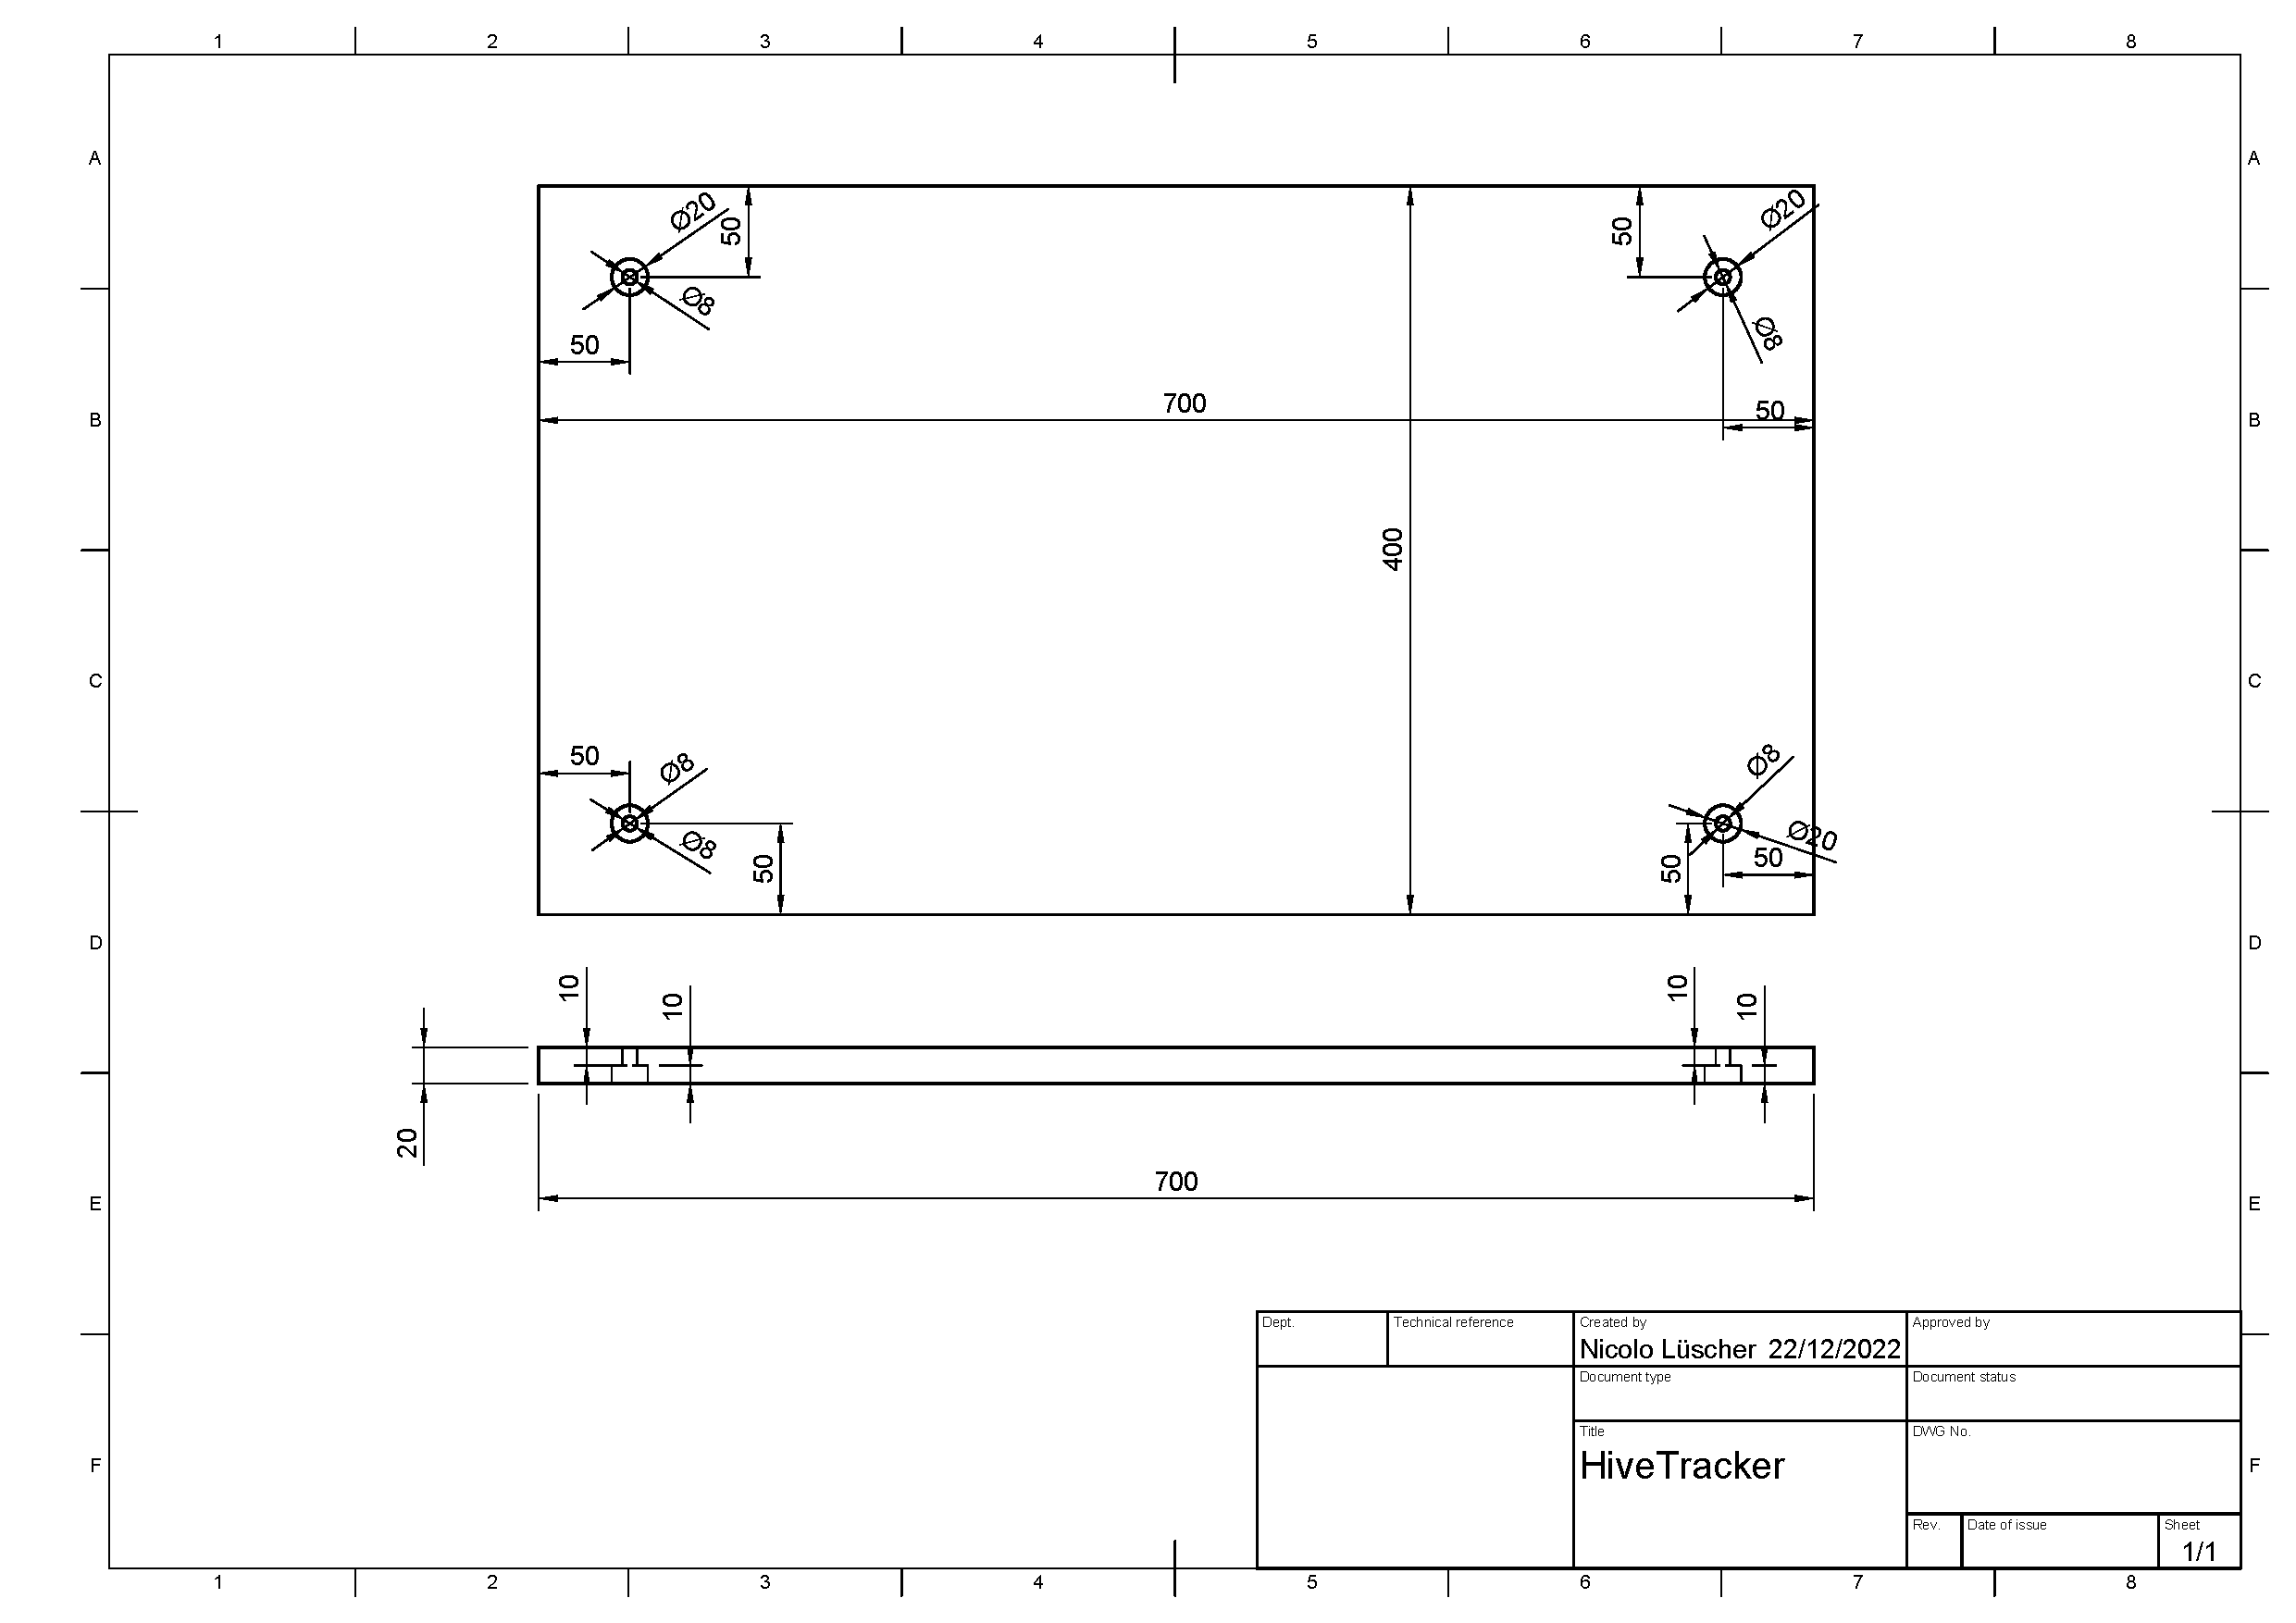
\includegraphics[angle=90,width=1\textwidth]{figures/hivetracker_baseplate.pdf}
    \caption{Baseplate Technical Drawing}
    \label{fig:baseplate_drawing}
\end{figure}
\newpage

\subsubsection{Load Cells}
The load cells used are a generic Chinese product normally used for human scales and are rated for 50 kg each. Since there are four of them, the maximum weight that can be measured is 200 kg. This is more than enough for a beehive.

\begin{figure}
    \centering
    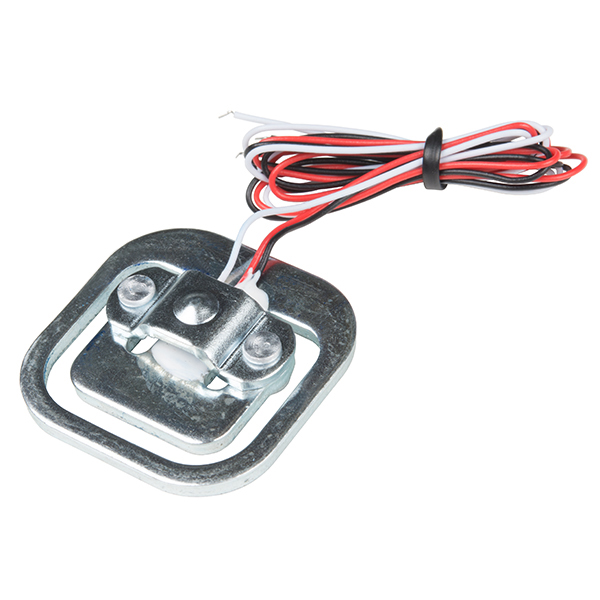
\includegraphics[width=0.5\textwidth]{figures/loadcell.jpg}
    \caption{Load Cell}
    \label{fig:loadcell}
\end{figure}

\newpage
\subsubsection{Load Cell Amplifier}
The load cells are connected to a HX711 load cell amplifier. It is used to read the measurements from the load cells and convert them into usable data. The amplifier is connected to the microcontroller.

\begin{figure}
    \centering
    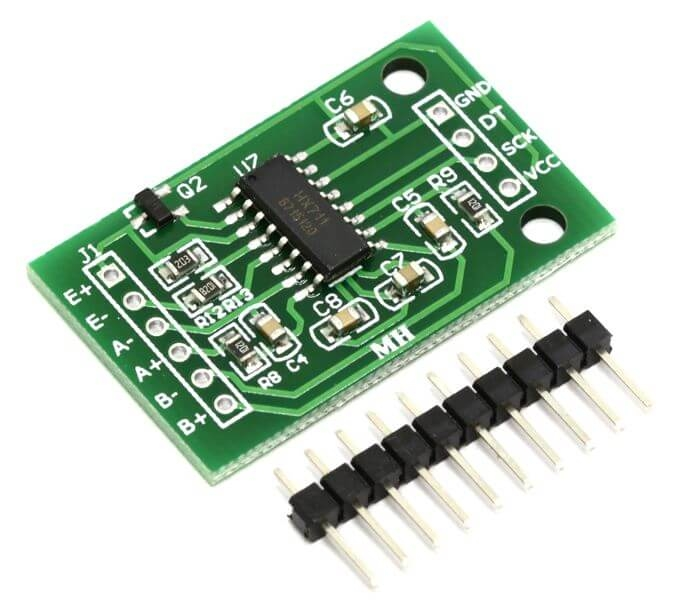
\includegraphics[width=0.5\textwidth]{figures/hx711.jpg}
    \caption{Load Cell Amplifier}
    \label{fig:loadcell_amplifier}
\end{figure}

\newpage
\subsubsection{Temperature Sensor}
The temperature sensor is a DS18B20 waterproof temperature sensor with a 3 m cable. It is connected to the microcontroller and can be used to measure the temperature inside the beehive.

\begin{figure}
    \centering
    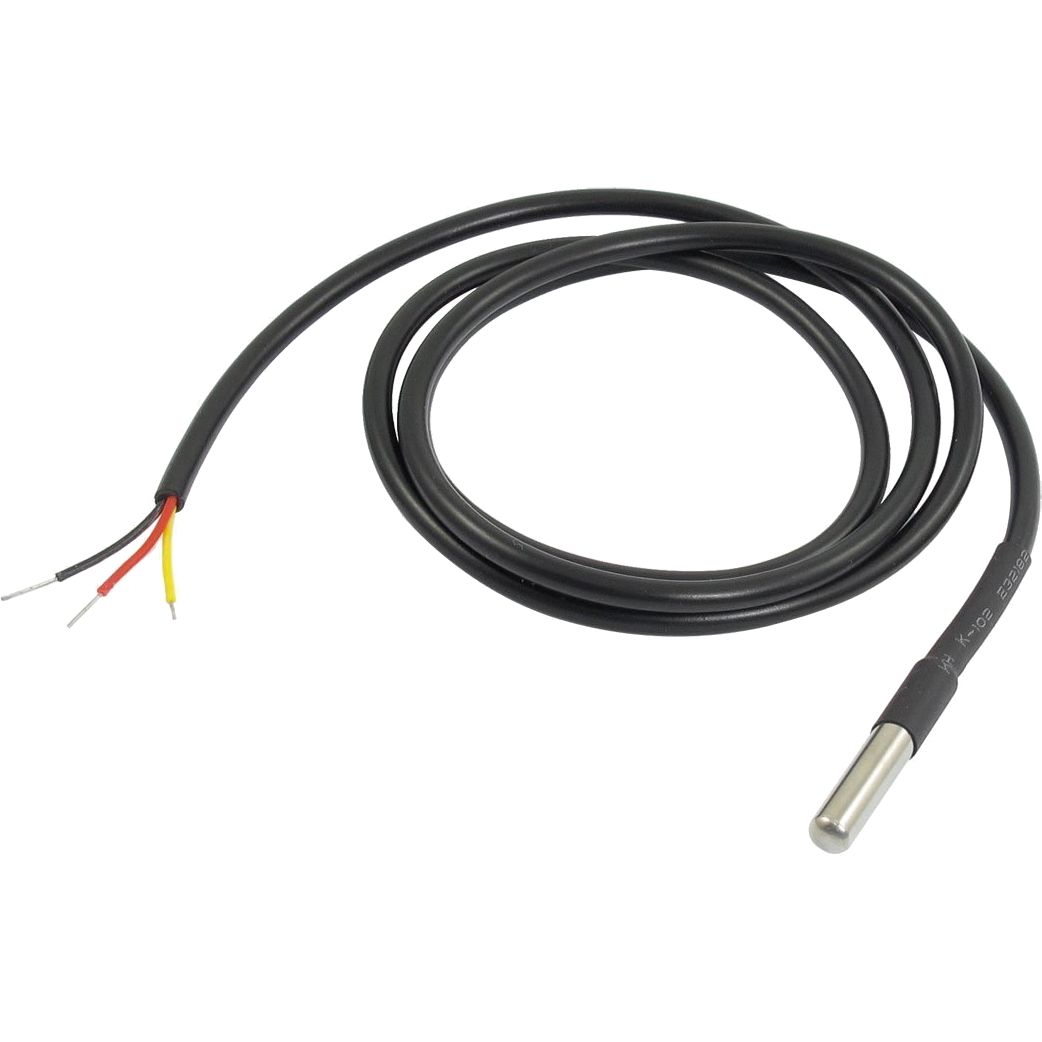
\includegraphics[width=0.5\textwidth]{figures/DS18B20.png}
    \caption{Temperature Sensor}
    \label{fig:temperature_sensor}
\end{figure}
\newpage
\subsubsection{Microcontroller}
The microcontroller is LILYGO® TTGO T-Call V1.4 ESP32 Wireless Module with a built-in SIM800L Module for GSM/GPRS. It is already capable to connect the internet via a SIM card out of the box, and it can be powered by a 3.3V - 5V DC power source, making it possible to use a wide variety of power sources. The documentation is quite poor, mostly consisting of a Chinese data sheet and a few examples. However, it is possible to use the Arduino IDE to program it, which makes it easy to use since all the necessary libraries to use the load cell amplifier and the temperature sensor are already included.

\begin{figure}
    \centering
    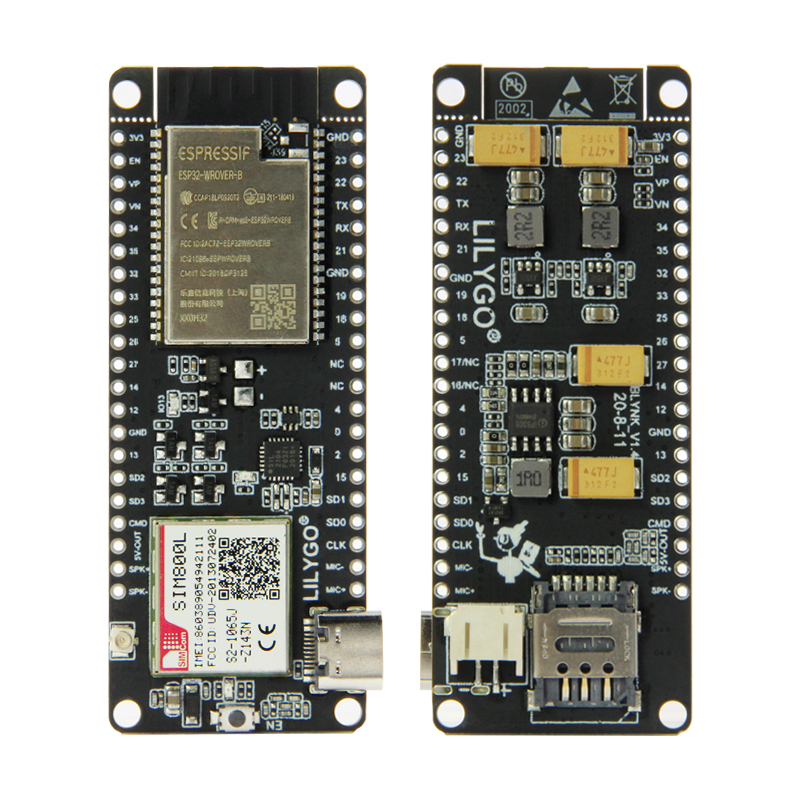
\includegraphics[width=0.5\textwidth]{figures/esp32.jpg}
    \caption{LILYGO® TTGO T-Call V1.4 ESP32 Wireless Module Microcontroller}
    \label{fig:esp32}
\end{figure}

\newpage
\subsection{Software Planning}

\subsubsection{Architecture}
The software is split into five different components. These components should be connected to each other via a simple interface, so that it is easy to replace any of them with a different implementation.
The components are:
\begin{itemize}
    \item Sensor Block
    \item Data Broker
    \item Backend
    \item Database
    \item User Interface
\end{itemize}

\begin{figure}
    \centering
    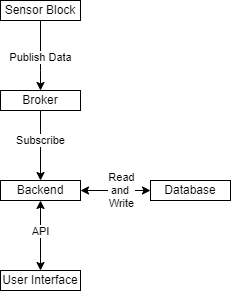
\includegraphics[width=0.5\textwidth]{figures/hivetracker_software_architecture.png}
    \caption{Software Architecture}
    \label{fig:software_architecture}
\end{figure}

\subsubsection{Sensor Block / ESP32 Firmware}
The sensor block runs the ESP32 firmware. The ESP32 firmware is written in C++ and uses the Arduino framework. It implements several libraries to interact with the hardware. Refer to section \ref{sec:firmware} for more information.

\subsubsection{Data Broker}
Data between the sensor block and the backend is exchanged via a data broker. The data broker is a simple MQTT broker. The sensor block publishes the data to the broker and the backend subscribes to this data. The data broker is implemented using the Mosquitto MQTT broker. Refer to section \ref{sec:data_broker} for more information.

\subsubsection{Backend}
The backend listens for data coming from the sensor block by subscribing to the data broker. If there is new data, it is timestamped and stored in the database. The backend also provides an API that can be used by the frontend to receive data from the database and make changes to the calibration information used to calibrate the scale. The backend is implemented using Node.js and Express. Refer to section \ref{sec:backend} for more information.

\subsubsection{Database}
The database is used to store all data related to the beehive. It makes the otherwise ephemeral data persistent and allows to query it. The database is implemented using Postgres. Refer to section \ref{sec:database} for more information.

\newpage
\section{Implementation}


\subsection{Prototype}
\subsubsection {Hardware} \label{sec:hardware}
The first step was to build the hardware of the prototype. For this I first had to build the scale itself.

For this I cut out the baseplates from wood according to my technical drawing and then drilled the required holes for the nuts and bolts. I then glued the load cells to the baseplates and wired them together as seen in figure \ref{fig:loadcell_wiring}. I had to drill some shallow relief holes I did not account for in my design because the load cells had a small protrusion and wouldn't have laid flush otherwise. Furthermore, I then connected the load cells to the load cell amplifier and the load cell amplifier to the microcontroller.

\begin{figure}
    \centering
    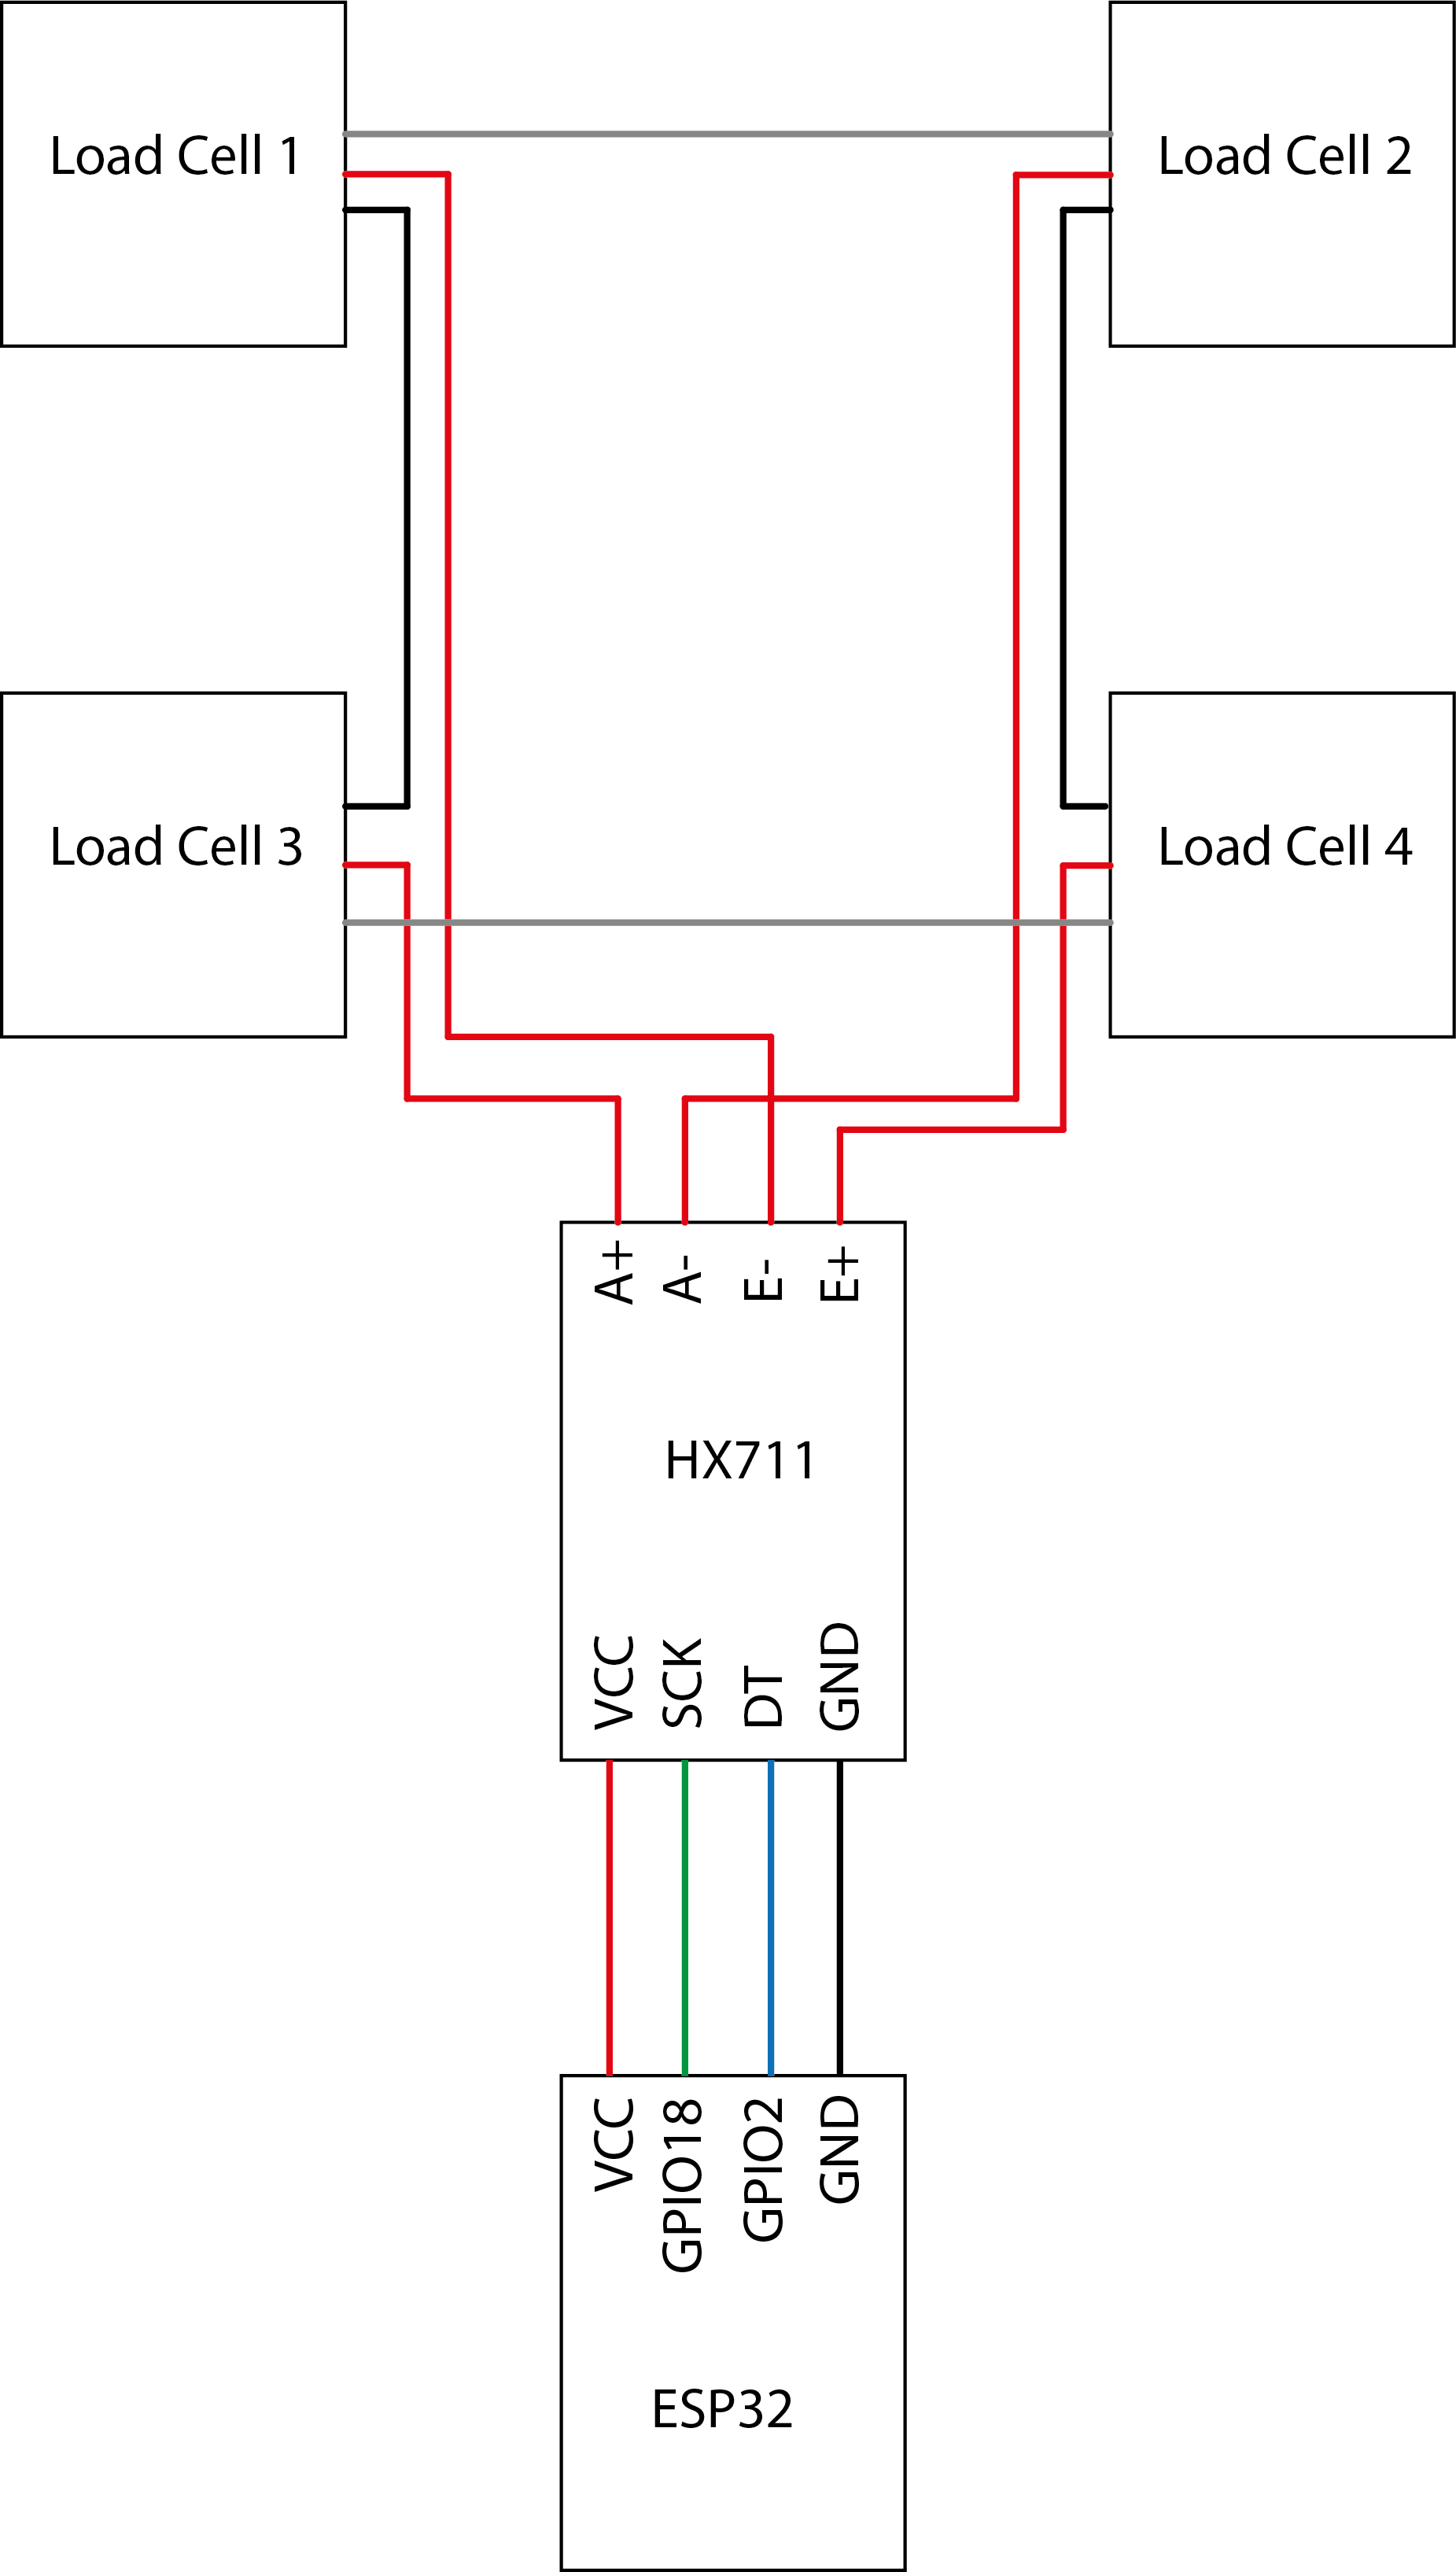
\includegraphics[width=0.5\textwidth]{figures/loadcell_wiring.png}
    \caption{Baseplate Prototype}
    \label{fig:loadcell_wiring}
\end{figure}

After that, I glued some squares cut from hard plastic and glued them to the baseplate without the load cells at the contact points of the load cells. This is to prevent the load cells from digging into the wood and to make sure that the load cells are not damaged by the wood. I then placed the two plates on top of each other and bolted them together.

I then tested the scale for accuracy and repeatability. I found that the scale was not suited for quick measurements, since it takes a few seconds for the load cells to settle. My guess is that this is due to stress in the wood. However, it is accurate enough for my purposes since I am interested in the change in weight over time, not the absolute weight at a given moment.

After this I connected the temperature sensor to the microcontroller. For this, I had to solder a 4.7 k\Omega resistor to the temperature sensor and connect it to the microcontroller as seen in figure \ref{fig:temperature_wiring}. I then tested the temperature sensor and found that it was very accurate.

\begin{figure}
    \centering
    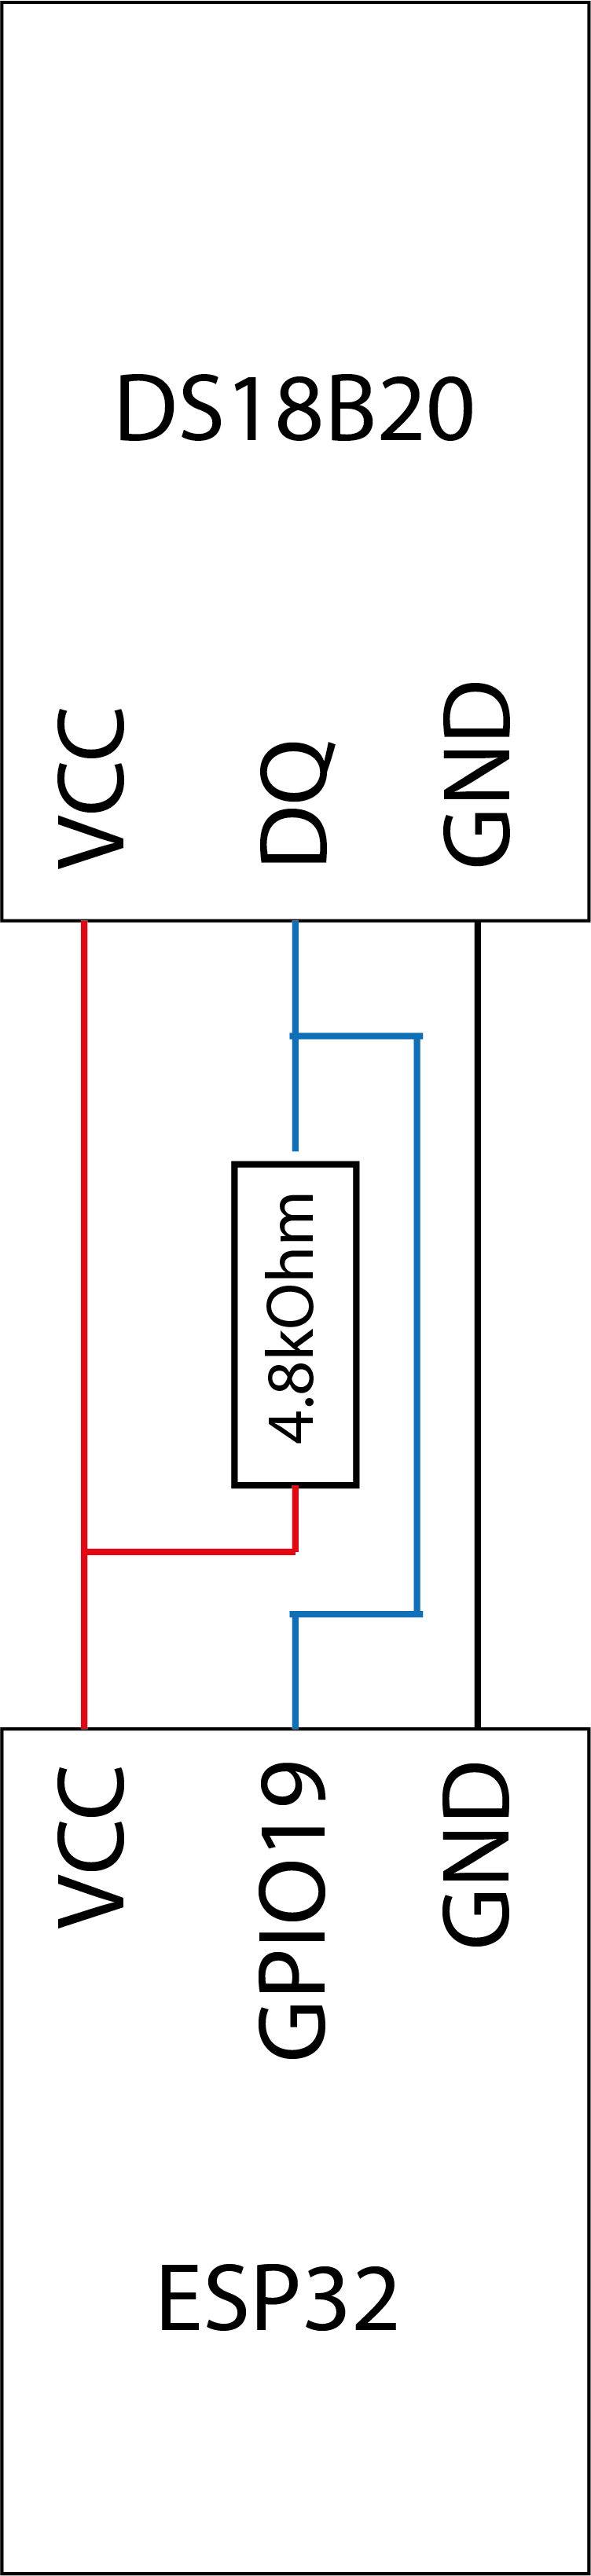
\includegraphics[angle=270,width=1\textwidth]{figures/temperature_wiring.png}
    \caption{Temperature Sensor Prototype}
    \label{fig:temperature_wiring}
\end{figure}

\newpage
\subsubsection {Firmware} \label{sec:firmware}
The firmware is written in C++ and uses the Arduino framework and is used to get the data from the sensors to the data broker.

Simplified, the firmware performs the following steps:

\begin{enumerate}
    \item Determine the board type and set up the hardware accordingly
    \item Set configuration values
    \item Establish a connection to the GSM network via the SIM800L module
    \item Set up a connection to the data broker via MQTT
    \item Initialize the temperature Sensor
    \item Initialize the load cell amplifier
    \item Read the Temperature
    \item Read the Weight
    \item Write the data to the data broker
    \item Disconnect from the data broker
    \item Disconnect from the GSM network
    \item Enter deep sleep mode for a given amount of time
    \item Wake up and repeat
\end{enumerate}

Refer to appendix \ref{lst:firmware} for the full source code of the firmware.

\subsection{Server Setup}
\subsubsection {Data Broker} \label{sec:data_broker}
For easy deployment, I decided to use a docker container for the data broker. I used the official Mosquitto docker image and configured it to use a password file for authentication. I also configured it to use TLS encryption. Refer to appendix \ref{lst:mosquitto-conf} for the configuration file and to appendix \ref{lst:mqtt-docker-compose} for the docker compose file.

This broker provides standard MQTT functionality and is used to exchange data between the sensor block and the backend. The sensor block publishes the data to a topic on the broker and the backend subscribes to this topic. This means that the backend automatically gets notified when new data is available and doesn't have to poll the broker for new data.

\subsubsection {Backend} \label{sec:backend}
The backend persists the data coming from the data broker and makes it available to the user interface. It is implemented using Node.js and Express. It uses the MQTT.js library to connect to the data broker and uses Sequelize to interact with the database. Refer to appendix \ref{sec:backend} for the relevant source code of the backend.

\textbf{Node.js} is a JavaScript runtime that allows to run JavaScript code outside the browser. This makes it possible to implement server side code in JavaScript. It also provides a package manager that allows to easily install and manage dependencies called NPM (Node Packet Manager). In this project, Node is used to handle incoming HTTP requests and to interact with the database. 
It exposes an API that allows to query the database and to retrieve the data to be displayed in the user interface. There are also endpoints that allow to update the configuration of the beehive. This includes a server side method to calibrate the scale and set a zero offset. Refer to appendix \ref{lst:app.js} for the relevant source code of the backend.

\textbf{Express.js} is a web framework for Node.js that allows to easily implement HTTP endpoints. It provides a simple API to define the endpoints and to handle incoming requests. It also provides a middleware system that allows to easily add functionality to the endpoints. Express.js provides an easy way to implement backend routing and greatly simplifies the code structure and the endpoint management.

\textbf{Sequelize} is an ORM (Object Relational Mapper) that allows to interact with the database using JavaScript objects. It provides a simple API to define the database schema and to interact with the database. It also provides a migration system that allows to easily update the database schema. This is useful for example when new data is added to the database or when the data format changes. It also allows to easily query the database and to retrieve the data in a format that is easy to use in the user interface without having to write any SQL queries. Refer to appendix \ref{lst:database.js} for the database schema.
Sequelize adds the "createdAt" and "updatedAt" field to any data entry by default and automatically updates them when the data is changed. This further simplifies the backend code.

\textbf{MQTT.js} is a library that allows to connect to an MQTT broker and to subscribe to topics. It also provides an API to publish data to a topic. It is used to connect to the data broker and to subscribe to the topic that the sensor block publishes to. The backend is then automatically notified when new data is available and can act accordingly.

\textbf{Networking}
The backend and the frontend are intended to be deployed on the same machine. To simplify the port management, a reverse proxy is used to route all API requests to the backend and all other requests to the frontend. This is done using the Angular reverse proxy. This allows the machine to only expose port 80 and 443 to the internet and handle the rest internally making it easier to implement TLS encryption.

\subsubsection {Database} \label{sec:database}
The database is used to store data related to the project. It is implemented using PostgreSQL and is managed using Sequelize. It is running in a docker container and is exposed to the backend via a docker network making it easy to deploy and manage. The same docker container is also running an Adminer instance that allows to easily manage the database. Refer to appendix \ref{lst:database-docker-compose.yml} for the docker compose file.

\begin{figure}
    \centering
    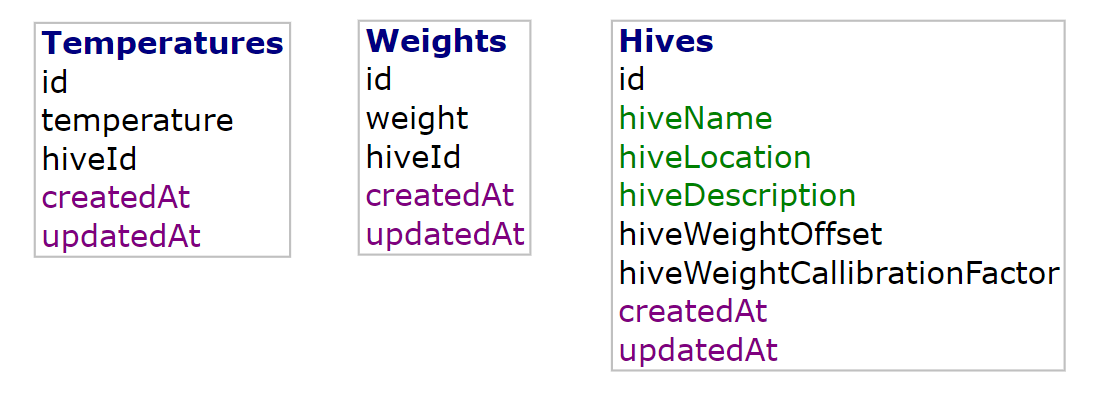
\includegraphics[width=0.75\textwidth]{figures/database_shema.png}
    \caption{Database Schema}
    \label{fig:database}
\end{figure}

The database schema is quite simple. It consists of three tables that store the relevant data.

\textbf{Temperatures} and \textbf{Weights} store the data coming from the sensors. They both have a \textbf{value} field that stores the actual data and a \textbf{createdAt} field that stores the timestamp when the data was created. The \textbf{updatedAt} field is automatically updated by Sequelize when the data is changed. This means that the data can be queried by the backend using the \textbf{createdAt} field and the backend can easily determine the time difference between two data points. They also both have a \textbf{hiveId} field that stores the ID of the beehive that the data belongs to. This allows for multiple beehives to be connected to the same database.

The \textbf{Hives} database stores information about a given hive. This includes administrative information like among other things a name to tell them apart and a location to determine where they are located. This might be used by a frontend to provide geodata or to collect additional data like weather. It also stores values that are used to calibrate the scale. This includes a \textbf{hiveWeightOffset} field that stores the offset that is used to zero the scale and a \textbf{hiveWeightCalibrationFactor} field that stores a factor used to calibrate the scale. This means that all the information needed to display the data from the beehive is stored on the database and the user interface doesn't have to do any calculations. This also allows the user to change the calibration of the scale at any time without having to do any changes to the scale itself.

\newpage
\subsection{User Interface}\label{sec:user_interface}
The system is designed to make it user interface agnostic. This means that the user interface can take any shape and form as long as it can interact with the backend over the provided API endpoints. This allows to easily implement different user interfaces for different use cases. For example, a user interface for a mobile phone and a user interface for a desktop computer. This also allows to easily implement different user interfaces for different users. For example, a user interface for the beekeeper and a user interface for the bee researcher.

The user interface I've implemented for this project is a simple web application that allows to view the data coming from the beehive. The user is also able to update the configuration of the beehive. This includes a method to calibrate the scale and set a zero offset and therefore provides all the functionality to set up the beehive.

The user interface is implemented using \textbf{Angular} and is deployed using the Angular reverse proxy. This is a bit overkill for this project, but it allows to easily extend the user interface in the future by providing a simple way to add new pages, components and services. For styling, \textbf{TailwindCSS} is used. It provides a simple, low CSS way to style the user interface with a result focused, fast approach.

\begin{figure}
    \centering
    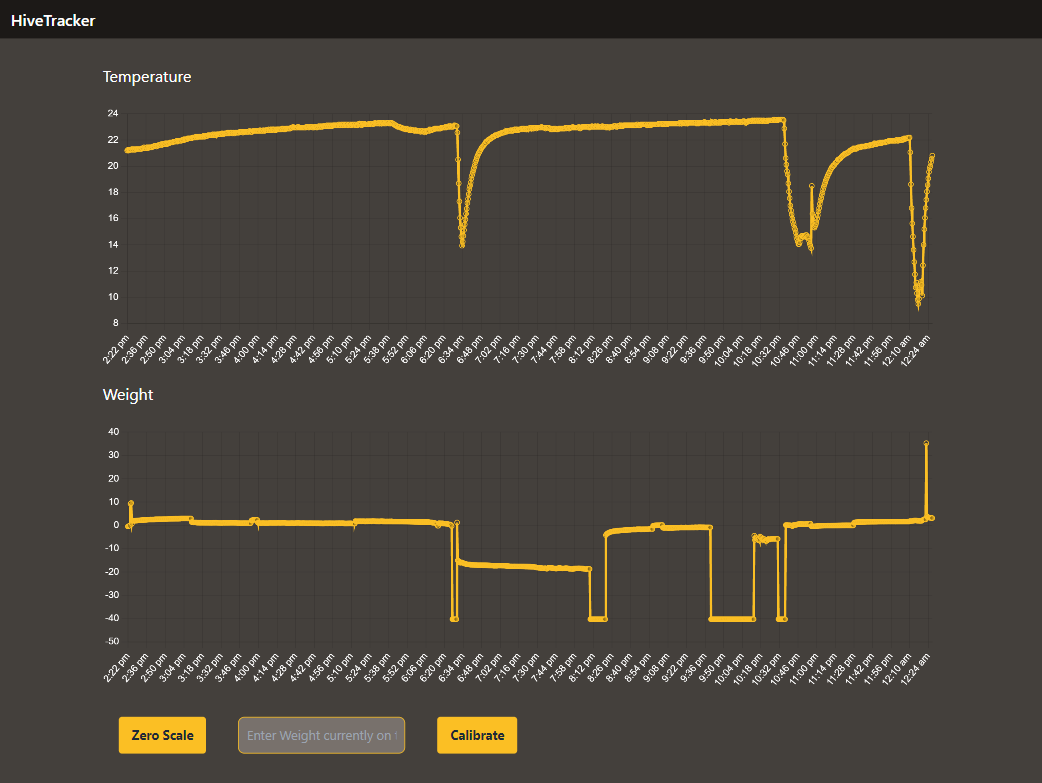
\includegraphics[width=0.8\textwidth]{figures/user_interface.png}
    \caption{Screenshot of the user interface}
    \label{fig:user_interface}
\end{figure}

\newpage
\section{Testing}
\subsection{Hardware Testing}
Testing the system was done by trying to change the measured weight and temperature values and observing the results. The results were then compared to the expected results. The expected results were determined by the expected behavior of the system. This was done by setting up the system and then randomly changing the ambient temperature and adding/removing weight from the scale. The result of one of those testing sessions can be seen in figure \ref{fig:user_interface}.

The results of those tests showed that the temperature measurements are very accurate and closely match the ambient temperature. There were no sudden inaccuracies or spikes in the temperature measurements. 

The weight measurements however showed a great degree of uncertainty and drift. The weight would drift up and down by several hundred grams without any changes to the scale itself. These drifts however correlated with other changing factors like temperature or time since the last weight change. This means that the weight measurements are not very accurate and can't be used to determine the weight of the beehive with a high degree of accuracy. This is most likely due to the fact that the scale is built from natural wood that experiences internal stresses and changes in weight over time \cite{wood_deformation}. Another potential error sources are the load cells themselves. Load cells are known for being influenced by temperature changes \cite{loadcell_temperature}. This effect is even greater on cheap, consumer grade load cells.

These inaccuracies can be mitigated in several ways. The wood could be replaced by a more thermally stable material like processed wood, metal or plastic. The inaccuracies of the load cells could be reduced by installing a reference load cell that measures a know weight and using the difference between the theoretical weight and the measured weight to compensate for the temperature changes. This however are not trivial changes and are out of scope for this project and will be left for future work.

\subsection{Power Consumption}
Power consumption is a very important factor in "off-grid" IOT systems. It determines the choice of power supply that is necessary to power the system.

To measure the power consumption, a USB power meter was hooked in between the power supply and the microcontroller. The power meter was then used to measure the voltage and current draw of the system.

\begin{figure}
    \centering
    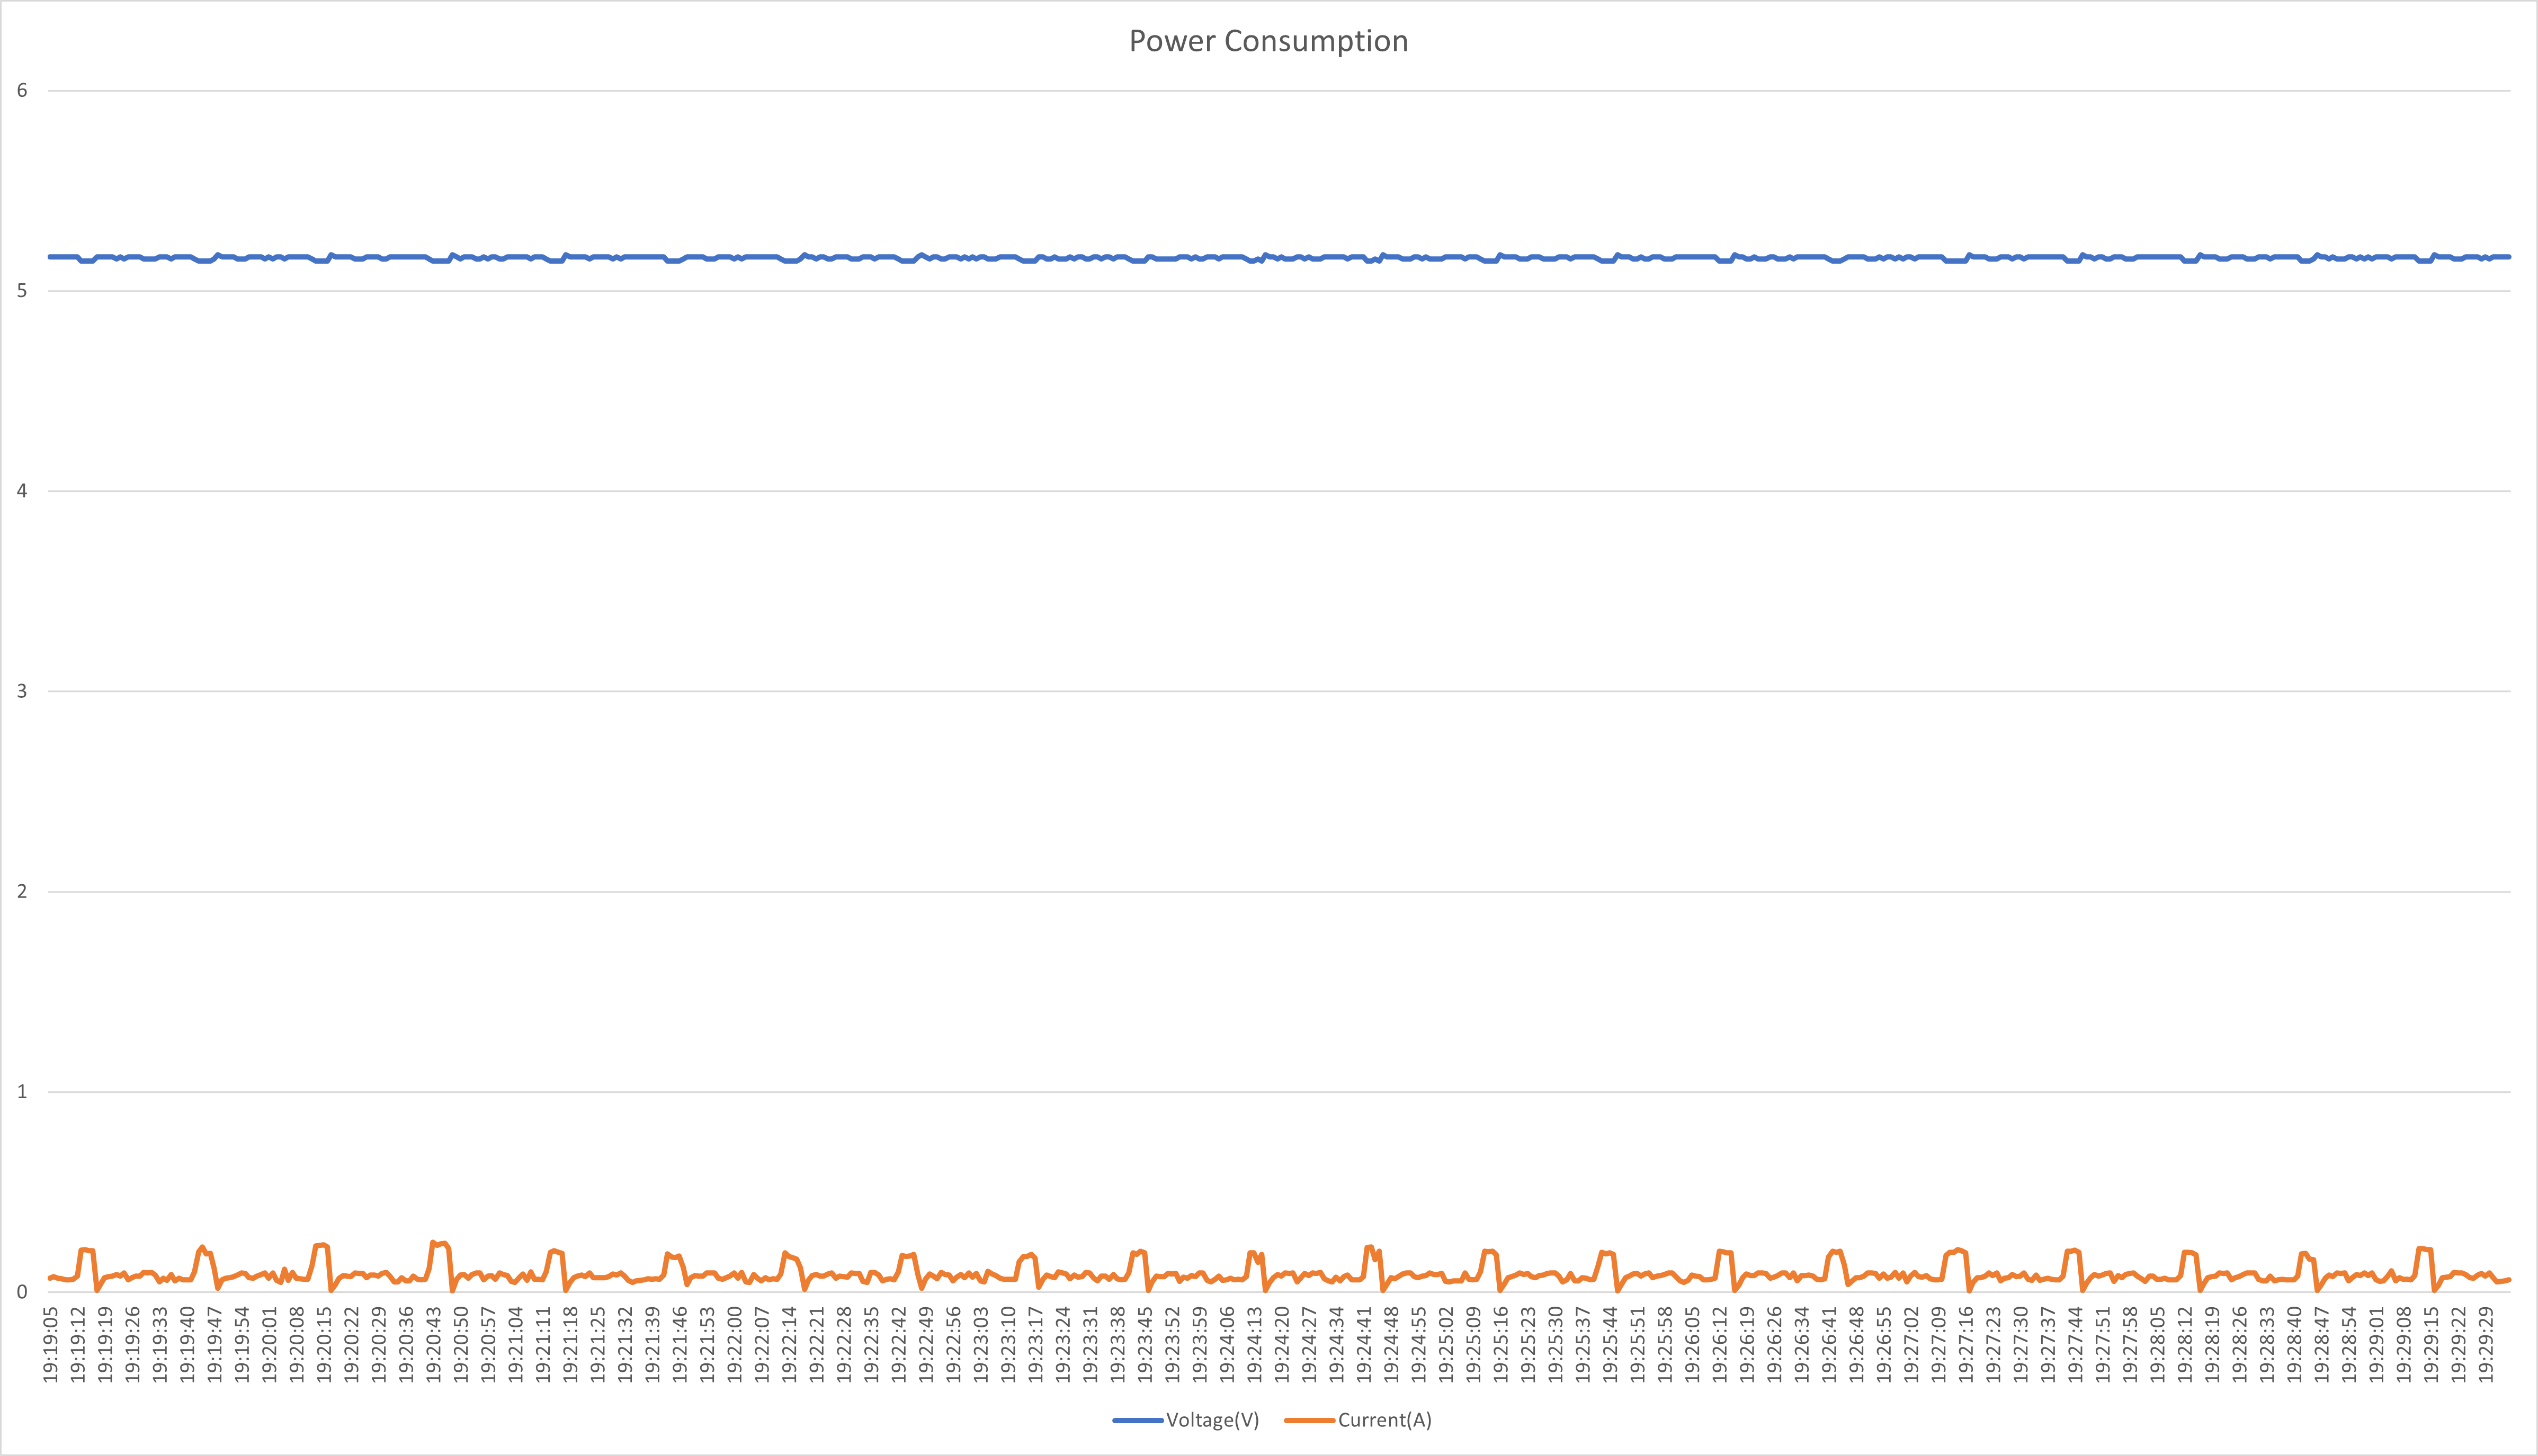
\includegraphics[width=1\textwidth]{figures/power_consumption_graph.png}
    \caption{Power consumption of the system over multiple measuring cycles}
    \label{fig:power_consumption}
\end{figure}
See \ref{lst:power-management} for the data used to generate the graph.

\subsubsection{Methodology}
The power meter used was a UM34C inline USB power meter. Measures the voltage and current draw of the USB port and saves it to a CSV file. The CSV file was then imported into a spreadsheet and the average current draw was calculated. The average current draw was then multiplied by the voltage to get the average power consumption.

The microcontroller was set to instantly restart after it has done one measuring cycle. This was done for a total of 20 cycles. The average current draw was then calculated from the 20 measurements. This was done to reduce the influence of the power supply on the measurements. The power supply used was a 5V 2A power supply. With this information the average power consumption of a single measuring cycle can be calculated.

The deep sleep current was too low to be measured by the power meter. Therefore, 150\mu A given in the datasheet \cite{espressif_esp32} was used. 

With an average current draw of 92mA and an average voltage of 5.16V, the average power consumption during a measuring cycle is 0.48W. With a cycle duration of about 30 seconds, the average power consumption per cycle is 0.0158Wh. This means that the system can complete about 770 cycles on a standard 18650 battery with a capacity of 12.2Wh. The power consumption during deep sleep is about 75mW  which is negligible compared to the power consumption during a measuring cycle. Those numbers show that the battery life of the system is limited by the battery capacity and the frequency of the measuring cycles.

With a setup of 4 18650 batteries and a cycle frequency of 1 cycle every 10 minutes, the system can run for about 21.4 days before the batteries need to be replaced. If we only take measurements every hour, which is what most beekeepers do, the system can run for about 128 days which means that the batteries only need to be replaced three times a year.

Adding solar panels to the system would enable it to run indefinitely. With a 10-minute measuring frequency, the system would have to be in direct sunlight every 21 days to keep the batteries charged. This should be more than enough for most beekeepers and would be a great future improvement to the system.


\subsection{Software Testing}
Due to the simplicity of the software, no automated testing were done. The software was tested manually by trying to interact with it and observing the results. The results were then compared to the expected results.

\subsubsection{Data Broker}
The data broker was tested with the \textbf{MQTT Explorer} client. This allows to connect to the broker directly and see what data is being published. This also allows to verify the TLS authentication. The network traffic was also monitored to verify that the data is being encrypted and no plain text information like usernames and passwords are being sent over the network unencrypted.

The broker satisfied all the requirements and was therefore considered to be working correctly.

\subsubsection{Backend}
The functionality of the backend was verified by exploring the API endpoints using \textbf{Postman}. This allowed to verify that the endpoints are working correctly and that the data is being stored correctly in the database. The subscription to the MQTT broker was also verified by using the MQTT Explorer client to publish data to the broker and observing the results in the backend.

The backend satisfied all the requirements and was therefore considered to be working correctly.

\subsubsection{Database}
The database was tested by accessing the database directly using the \textbf{Adminer} web application and verifying that the tables were set up correctly by Sequelize and that the data was being stored correctly. The database was also verified by using the API endpoints and observing if the data was being stored correctly.

The database satisfied all the requirements and was therefore considered to be working correctly.

\subsubsection{User Interface}
The user interface was tested by using it to interact with the system and testing the different features. This included testing the different API endpoints and observing the results. For example by testing the calibration of the scale and observing if the zero offset was being set and the scale was being calibrated correctly.

The user interface was also tested on different devices to verify that it is responsive and works correctly on different screen sizes.

The user interface satisfied all the requirements and was therefore considered to be working correctly.
\Gls{BibTeX}